\begin{titlepage}
\thispagestyle{empty}
\definecolor{covernavy}{HTML}{0F2A4A}
\definecolor{coveraccent}{HTML}{F2A33A}
\begin{tikzpicture}[remember picture,overlay]
  \fill[covernavy] (current page.south west) rectangle (current page.north east);
  \node[anchor=south,inner sep=0pt] at (current page.south) {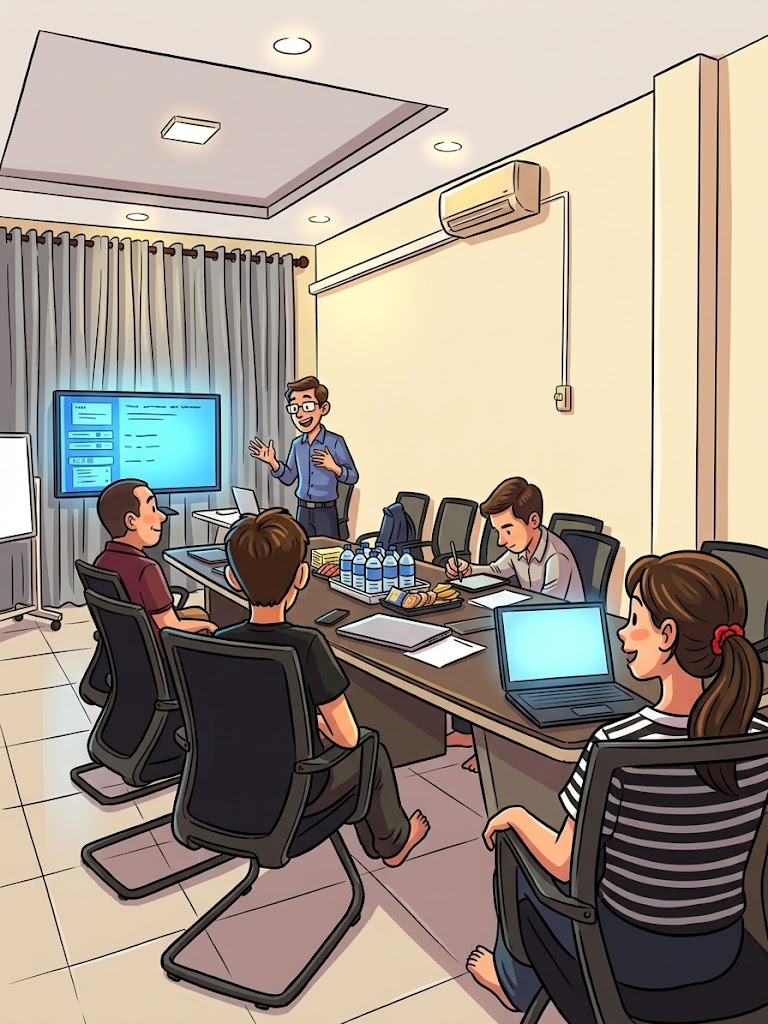
\includegraphics[width=\paperwidth]{figures/provided/cover-class-illustration.png}};
  \fill[covernavy] (current page.north west) rectangle ([yshift=-10.6cm]current page.north east);
  \fill[coveraccent] ([yshift=-1.6cm]current page.north west) rectangle ([yshift=-1.85cm]current page.north east);
  \node[anchor=north,text=white,align=center,text width=17cm] at ([yshift=-2.7cm]current page.north)
     {\centering{\fontsize{14}{18}\selectfont\textcolor{coveraccent}{\textsc{Build Your Own AI \textperiodcentered{} Grades 7--12}}\par}\vspace{7mm}
      {\fontsize{40}{46}\selectfont\bfseries\spaceskip=0.33em plus 0.1em No-code AI for Young Cambodian Learners\par}\vspace{6mm}
      {\fontsize{15}{20}\selectfont A hands-on guide to building AI with Google Teachable Machine\par}};
  \fill[covernavy,opacity=0.9] (current page.south west) rectangle ([yshift=3.2cm]current page.south east);
  \node[anchor=center,text=white,align=center] at ([yshift=1.9cm]current page.south)
     {\fontsize{22}{26}\selectfont\bfseries Rina Buoy, PhD};
  \node[anchor=south,text=white!70,align=center] at ([yshift=0.5cm]current page.south)
     {\small Draft edition};
  \node[anchor=west,inner sep=0pt] at ([xshift=1.8cm,yshift=1.7cm]current page.south west) {
\includegraphics[height=1.9cm]{figures/provided/rinai-logo.png}};
  \node[anchor=east,text=white!80,align=right] at ([xshift=-1.8cm,yshift=1.7cm]current page.south east) {\small RinAI Academy\\ academy.rinabuoy.com};
\end{tikzpicture}
\end{titlepage}
\clearpage
\thispagestyle{empty}
\null\vfill
{\small\noindent\textbf{No-code AI for Young Cambodian Learners}\\ \copyright{} Rina Buoy, PhD. Draft edition.\\ Course website: \url{https://academy.rinabuoy.com}\\ Cover illustration and author photo: courtesy of the author.\\[6pt]
\textbf{Disclaimer.} This book was prepared with the assistance of Claude Code, an AI tool from Anthropic. The author provides the content and reviews and revises all of the outputs.}
\clearpage

